\usepackage{xcolor}
\usepackage{afterpage}
\usepackage{pifont,mdframed}
\usepackage[bottom]{footmisc}

\usepackage{amsmath}
\usepackage{amsthm}
\usepackage{amssymb}
\usepackage{mathtools}


\createsection{\Grader}{Grader di prova}

\newcommand{\inputfile}{\texttt{stdin}}
\newcommand{\outputfile}{\texttt{stdout}}

\newenvironment{warning}
  {\par\begin{mdframed}[linewidth=2pt,linecolor=gray]%
    \begin{list}{}{\leftmargin=1cm
                   \labelwidth=\leftmargin}\item[\Large\ding{43}]}
  {\end{list}\end{mdframed}\par}

% % % % % % % % % % % % % % % % % % % % % % % % % % % % % % % % % % % % % % % % % % %
% % % % % % % % % % % % % % % % % % % % % % % % % % % % % % % % % % % % % % % % % % %


Si calcoli il minimo albero ricoprente di un grafo pesato non orientato avente $N$ nodi e $M$ archi.


% % % % % % % % % % % % % % % % % % % % % % % % % % % % % % % % % % % % % % % % % % %
% % % % % % % % % % % % % % % % % % % % % % % % % % % % % % % % % % % % % % % % % % %

\Implementation

Dovrai sottoporre un unico file, con estensione \texttt{.cpp}.

\begin{warning}
Tra gli allegati a questo task troverai un template \texttt{mst.cpp} con un esempio di implementazione.
\end{warning}

Dovrai implementare la seguente funzione:

\begin{center}\begin{tabularx}{\textwidth}{|c|X|}
\hline
C++  & \verb|int mst(int N, int M, int A[], int B[], int P[], int C[], int D[]);|\\
\hline
\end{tabularx}\end{center}

\begin{itemize}[nolistsep]
  \item L'intero $N$ rappresenta il numero di vertici del grafo.
  \item L'intero $M$ rappresenta il numero di archi del grafo.
  \item Gli array \texttt{A}, \texttt{B} e \texttt{P}, indicizzati da $0$ a $M-1$, dicono che esiste un arco che collega i vertici \texttt{A[$i$]} e \texttt{B[$i$]} avente peso \texttt{P[$i$]} per $i = 0, \ldots, M-1$.
  \item Gli array \texttt{C} e \texttt{D}, indicizzati da $0$ a $N-2$, sono inizialmente vuoti, e la funzione \texttt{mst} deve metterci gli archi di un albero ricoprente di costo minimo (l'$i$-esimo arco preso è quello che collega \texttt{C[$i$]} e \texttt{D[$i$]}).
  \item La funzione deve restituire la somma massima ottenibile.
\end{itemize}

\medskip

Il grader chiamerà la funzione \texttt{mst} e stamperà sul file di output il valore restituito e gli archi della soluzione trovata.

% % % % % % % % % % % % % % % % % % % % % % % % % % % % % % % % % % % % % % % % % % %
% % % % % % % % % % % % % % % % % % % % % % % % % % % % % % % % % % % % % % % % % % %


\Grader
Nella directory relativa a questo problema è presente una versione semplificata del grader usato durante la correzione, che potete usare per verificare le vostre soluzioni in locale. Il grader di esempio legge i dati da \inputfile{}, chiama le funzioni che dovete implementare e scrive su \outputfile{}, secondo il seguente formato.

Il file di input è composto da  $N+1$ righe, contenenti:
\begin{itemize}[nolistsep,itemsep=2mm]
\item Riga $1$: gli interi $N$ e $M$.
\item Righe $2, \ldots, M+1$: l'$i$-esima di queste righe contiene i valori \texttt{A[$i$]}, \texttt{B[$i$]} e \texttt{P[$i$]}.
\end{itemize}

Il file di output è composto da $N$ righe, contenenti:
\begin{itemize}[nolistsep,itemsep=2mm]
\item Riga $1$: il valore restituito dalla funzione \texttt{mst}.
\item Righe $2, \ldots, M+1$: l'$i$-esima di queste righe contiene i valori \texttt{C[$i$]} e \texttt{D[$i$]}, $i=0, \ldots, N-2$.
\end{itemize}

% % % % % % % % % % % % % % % % % % % % % % % % % % % % % % % % % % % % % % % % % % %
% % % % % % % % % % % % % % % % % % % % % % % % % % % % % % % % % % % % % % % % % % %


\Constraints

\begin{itemize}[nolistsep, itemsep=2mm]
	\item $1 \le N \le 10\,000$.
	\item $1 \le M \le 1\,000\,000$.
	\item $1 \le \texttt{P}[i] \le 10\,000$ per $i = 0, \ldots, M-1$.
	\item I vertici sono numerati da $0$ a $N-1$.
\end{itemize}

% % % % % % % % % % % % % % % % % % % % % % % % % % % % % % % % % % % % % % % % % % %
% % % % % % % % % % % % % % % % % % % % % % % % % % % % % % % % % % % % % % % % % % %

\Scoring

Il tuo programma verrà verificato su diversi test case raggruppati in subtask. Per ottenere il punteggio relativo a un subtask, è necessario risolvere correttamente tutti i test che lo compongono.

\begin{itemize}[nolistsep,itemsep=2mm]
  \item \textbf{\makebox[2cm][l]{Subtask 1} [\phantom{1}0 punti]}: Caso d'esempio.
  \item \textbf{\makebox[2cm][l]{Subtask 2} [15 punti]}: tutti gli archi hanno lo stesso peso.
  \item \textbf{\makebox[2cm][l]{Subtask 3} [15 punti]}: $N\leq 10, M\leq 20$.
  \item \textbf{\makebox[2cm][l]{Subtask 4} [20 punti]}: $M=N$.
  \item \textbf{\makebox[2cm][l]{Subtask 5} [50 punti]}: Nessuna limitazione specifica.
\end{itemize}

% % % % % % % % % % % % % % % % % % % % % % % % % % % % % % % % % % % % % % % % % % %
% % % % % % % % % % % % % % % % % % % % % % % % % % % % % % % % % % % % % % % % % % %


\Examples

\begin{example}
\exmpfile{mst.input0.txt}{mst.output0.txt}%
\end{example}

% % % % % % % % % % % % % % % % % % % % % % % % % % % % % % % % % % % % % % % % % % %
% % % % % % % % % % % % % % % % % % % % % % % % % % % % % % % % % % % % % % % % % % %


\Explanation

Il caso di esempio è rappresentato dalla figura seguente.
\begin{figure}[ht]
	\centering
	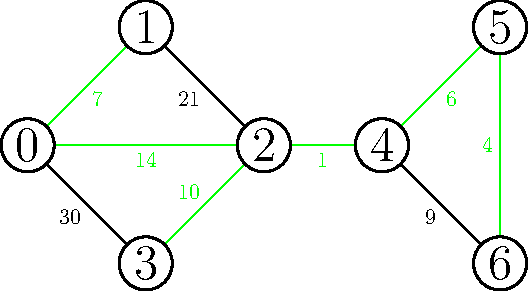
\includegraphics[scale = 0.8]{asy_mst/mst.pdf}
\end{figure}


